The given equation can be represented as follows in the vector form
%
\begin{align}
\vec{x}^T 
\myvec{
1 & 0 \\
0 & 0
}
\vec{x} + 
\myvec{
0 & 0 
}
\vec{x} + 2 = 0
\end{align}
where,
\begin{align}
\vec{x} &= \myvec{x\\0}\\
x^2 + 2 &= 0\\
\implies  x^2 &= -2
\end{align}
Thus, the equation has no real roots as can be seen from Fig. \ref{sep/2/21/plot}
\begin{figure}[!ht]
\centering
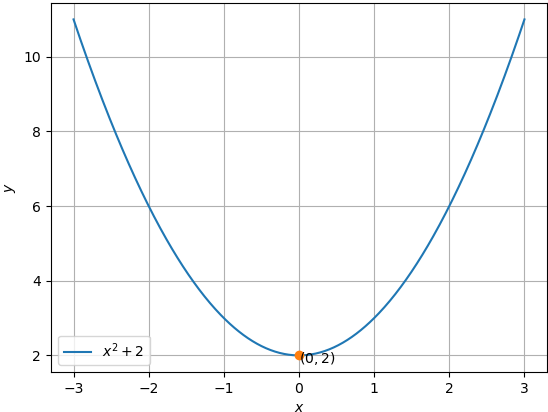
\includegraphics[width=\columnwidth]{solutions/sep/2/21/Figures/plot.png}
\caption{$x^2+2$ generated using python}
\label{sep/2/21/plot}
\end{figure} 

